\documentclass[10pt,a4paper]{article}

% Marges du document %
\setlength{\topmargin}{0cm}
\setlength{\headheight}{0.4cm}
\setlength{\headsep}{0.8cm}
\setlength{\footskip}{1cm}
\setlength{\textwidth}{17cm}
\setlength{\textheight}{25cm}
\setlength{\voffset}{-1.5cm}
\setlength{\hoffset}{-0.5cm}
\setlength{\oddsidemargin}{0cm}
\setlength{\evensidemargin}{0cm}

\usepackage{amssymb}
\usepackage{psfrag}
\usepackage[utf8]{inputenc}
\usepackage[francais]{babel}
\usepackage[T1]{fontenc}
\usepackage{amsmath}
\usepackage{amsfonts}
\usepackage{amssymb}
\usepackage{graphicx}
\usepackage{subcaption}
\usepackage{fancyhdr}
\usepackage{multicol}
\usepackage{eurosym} % symbole €
\usepackage{siunitx}
\usepackage{stmaryrd}
\usepackage{bm}

\usepackage{tabu}
\def\€{\euro{}}

\numberwithin{equation}{section}

\newcommand\numberthis{\addtocounter{equation}{1}\tag{\theequation}} 

\usepackage{color} % gestion de différentes couleurs
\definecolor{linkcolor}{rgb}{0,0,0}
\definecolor{linkcolorurl}{rgb}{0,0,1}
\usepackage[ pdftex,colorlinks=true,
pdfstartview=FitV,
linkcolor= linkcolor,
citecolor= linkcolor,
urlcolor= linkcolorurl,
hyperindex=true,
hyperfigures=false]
{hyperref} % fichiers pdf 'intelligents', avec des liens entre les références, etc.

% En-tête et pied de page % 
\pagestyle{fancy}
\fancyhead[L]{\scriptsize \textsc{Titre}} 
\fancyhead[R]{\scriptsize \textsc{BUNEL Félix et VERGNET Hadrien}} 
\fancyfoot[C]{ \thepage}

\author{Bunel Félix et Vergnet Hadrien}

%%%%%%%%%%%%%%%%%%%%%%%%%%%%%
% Tikz packages and settings
%%%%%%%%%%%%%%%%%%%%%%%%%%%%%

\usepackage{tikz}
\usepackage{pgfplots}
\usepackage{tikz-3dplot}
\pgfplotsset{compat=1.11}

\usetikzlibrary{shapes.geometric,calc,intersections}
\usetikzlibrary{shapes.arrows}
\usetikzlibrary{shadings}
\usetikzlibrary{patterns}
\usetikzlibrary{decorations.pathmorphing}
\usetikzlibrary{decorations.pathreplacing}


\usetikzlibrary{external}
\tikzset{external/aux in dpth={false}}
\tikzset{external/up to date check={simple}}
\tikzset{external/optimize command away={\includetexgraphics}{2}}

\tikzset{>=stealth}

%%%%%%%%%%%%%%%%%%%%%%%%%%%%%%%%%%%%%%%%%%%%%%%%%%%%%%%%%%%%
% Custom macro to input a tikz picture and setting its name
%%%%%%%%%%%%%%%%%%%%%%%%%%%%%%%%%%%%%%%%%%%%%%%%%%%%%%%%%%%%

\makeatletter
\newcommand{\includetikzgraphics}[1]{
	\filename@parse{#1}
	\tikzsetnextfilename{\filename@base}
	\input{#1}
}
\makeatother

%%%%%%%%%%%%%%%%%%%%%%%%%%%%%%%%%%
% Custom tikz command for drawing
%%%%%%%%%%%%%%%%%%%%%%%%%%%%%%%%%%

\tikzset{math3d/.style=
    {z= {(-0cm,-0.3cm)}, y={(0cm,1cm)},x={(1cm,0cm)}}}

% \drawYNema {x} {y} {yAngle}
\newcommand{\drawYnema}[3] {
	\shade [ball color=black] (#1,#2) ellipse 
		[x radius={sqrt(pow(cos(#3)*0.1,2)+pow(sin(#3)*0.3,2))}, y radius=0.1];
}
% \drawXNema {x} {y} {xAngle}
\newcommand{\drawXnema}[3] {
	\shade [ball color=black] (#1,#2) ellipse 
		[y radius={sqrt(pow(cos(#3)*0.1,2)+pow(sin(#3)*0.3,2))}, x radius=0.1];
}
% \drawZNema {x} {y} {zAngle}
\newcommand{\drawZnema}[3] {
	\shade [ball color=black] (#1,#2) ellipse 
		[x radius=0.3, y radius=0.1, rotate={#3}];
}

% \plotcylinder { radius } { heigth } { altitude }
\newcommand{\plotcylinder}[3] {
     \draw [math3d, fill=white, samples=100]
        plot[domain=-pi:pi] ({#1*cos(\x r)},#3,{#1*sin(\x r)}) ;
     \draw [math3d, fill=white, samples=100]
        plot[domain=0:pi] ({#1*cos(\x r)},#3,{#1*sin(\x r)}) --
        plot[domain=pi:0] ({#1*cos(\x r)},{#3-#2},{#1*sin(\x r)}) --
        cycle;
}

% \plotpolarizer { x} { y} { z } { radius } { angle }
\newcommand{\plotpolarizer}[5] {
    \draw [math3d, fill=gray, opacity=0.8, samples=100]
        plot[domain=-pi:pi] ({#1+#4*cos(\x r)},#2,{#3+#4*sin(\x r)}) ;
    \draw [math3d, opacity=0.8]
        ({#1+#4*cos(#5)},#2,{#3+#4*sin(#5)}) -- ({#1-#4*cos(#5)},#2,{#3-#4*sin(#5)}) ;
}

% \fancyarrow {xi} {yi} {xf} {yf} {width} {options}
\newcommand{\fancyarrow}[6]{
	\pgfmathsetmacro{\dx}{#3-#1};
	\pgfmathsetmacro{\dy}{#4-#2};
	\pgfmathsetmacro{\dl}{sqrt(\dx*\dx+\dy*\dy)};
	\pgfmathsetmacro{\dw}{#5/2};
	\pgfmathsetmacro{\cos}{\dx/\dl};
	\pgfmathsetmacro{\sin}{\dy/\dl};
	\draw [#6] (#1,#2) -- ++($\dw*(\sin,-\cos)$) 
		-- ++(${\dl-2*\dw}*(\cos,\sin)$)
		-- ++($\dw*(\sin,-\cos)$) -- ++($2*\dw*(\cos,\sin)+2*\dw*(-\sin,\cos)$) 
		-- ++($-2*\dw*(\cos,\sin)+2*\dw*(-\sin,\cos)$) -- ++($\dw*(\sin,-\cos)$)
		-- ++(${2*\dw-\dl}*(\cos,\sin)$) -- cycle;
}

%%%%%%%%%%%%%%%%%%%%%%%
% Custom pgf mark list
%%%%%%%%%%%%%%%%%%%%%%%
\pgfplotscreateplotcyclelist{colorhollowmarks}{%
	{black,mark=x},
	{cyan,mark=+},
	{magenta,mark=o},
	{teal,mark=square},
	{violet,mark=triangle},
	{gray,mark=diamond},
	{brown,mark=pentagon},
	{orange,mark=otimes},
	{lime,mark=10-pointed star}}
\pgfplotscreateplotcyclelist{hollowmarks}{%
	{mark=x},
	{mark=+},
	{mark=o},
	{mark=square},
	{mark=triangle},
	{mark=diamond},
	{mark=pentagona},
	{mark=otimes},
	{mark=10-pointed star}}
\pgfplotscreateplotcyclelist{onlycolors}{%
	black,
	cyan,
	magenta,
	teal,
	violet,
	lightgray,
	brown,
	orange,
	lime}



\begin{document}

%%%%%%%%%%%%%%%%%%%%%%%%%%%%%%%%%%%%%%%%%%%%%%%%%%%%%%%%%%%%%%%%%%%%%%%%%%%%%%%%%%%%%%%%
%%%%%%%%%%%%%%%%%%%%%%%%%%%%%%%%%%%%%%%%%%%%%%%%%%%%%%%%%%%%%%%%%%%%%%%%%%%%%%%%%%%%%%%%
\begin{titlepage}
%%%%%%%%%%%%%%%%%%%%%%%%%%%%%%%%%%%%%%%%%%%%%%%%%%%%%%%%%%%%%%%%%%%%%%%%%%%%%%%%%%%%%%%%
%%%%%%%%%%%%%%%%%%%%%%%%%%%%%%%%%%%%%%%%%%%%%%%%%%%%%%%%%%%%%%%%%%%%%%%%%%%%%%%%%%%%%%%%
\thispagestyle{empty}
\setlength{\parindent}{0pt}


\includegraphics[height=1.9cm]{logo-ens.jpg} \hfill 
\includegraphics[height=2cm]{logo_lyon1.jpg} \hfill 
\includegraphics[height=2cm]{logo_univ_lyon.jpg}



Master Sciences de la matière
\hfill
Projet de Géophysique

\textit{École Normale Supérieure de Lyon}
\hfill
BUNEL Félix et VERGNET Hadrien

\textit{Université Claude Bernard Lyon 1}
\hfill
M2 Physique 2015-2016
\vspace{0.5cm}

\hrulefill
\vspace{-0.6cm}

\hrulefill
\begin{center}\bfseries
\begin{huge}
    Titre
\end{huge}
\Large
\vspace{0.4cm}

Sous-titre
\end{center}
\hrulefill
\vspace{-0.6cm}

\hrulefill


\begin{center}
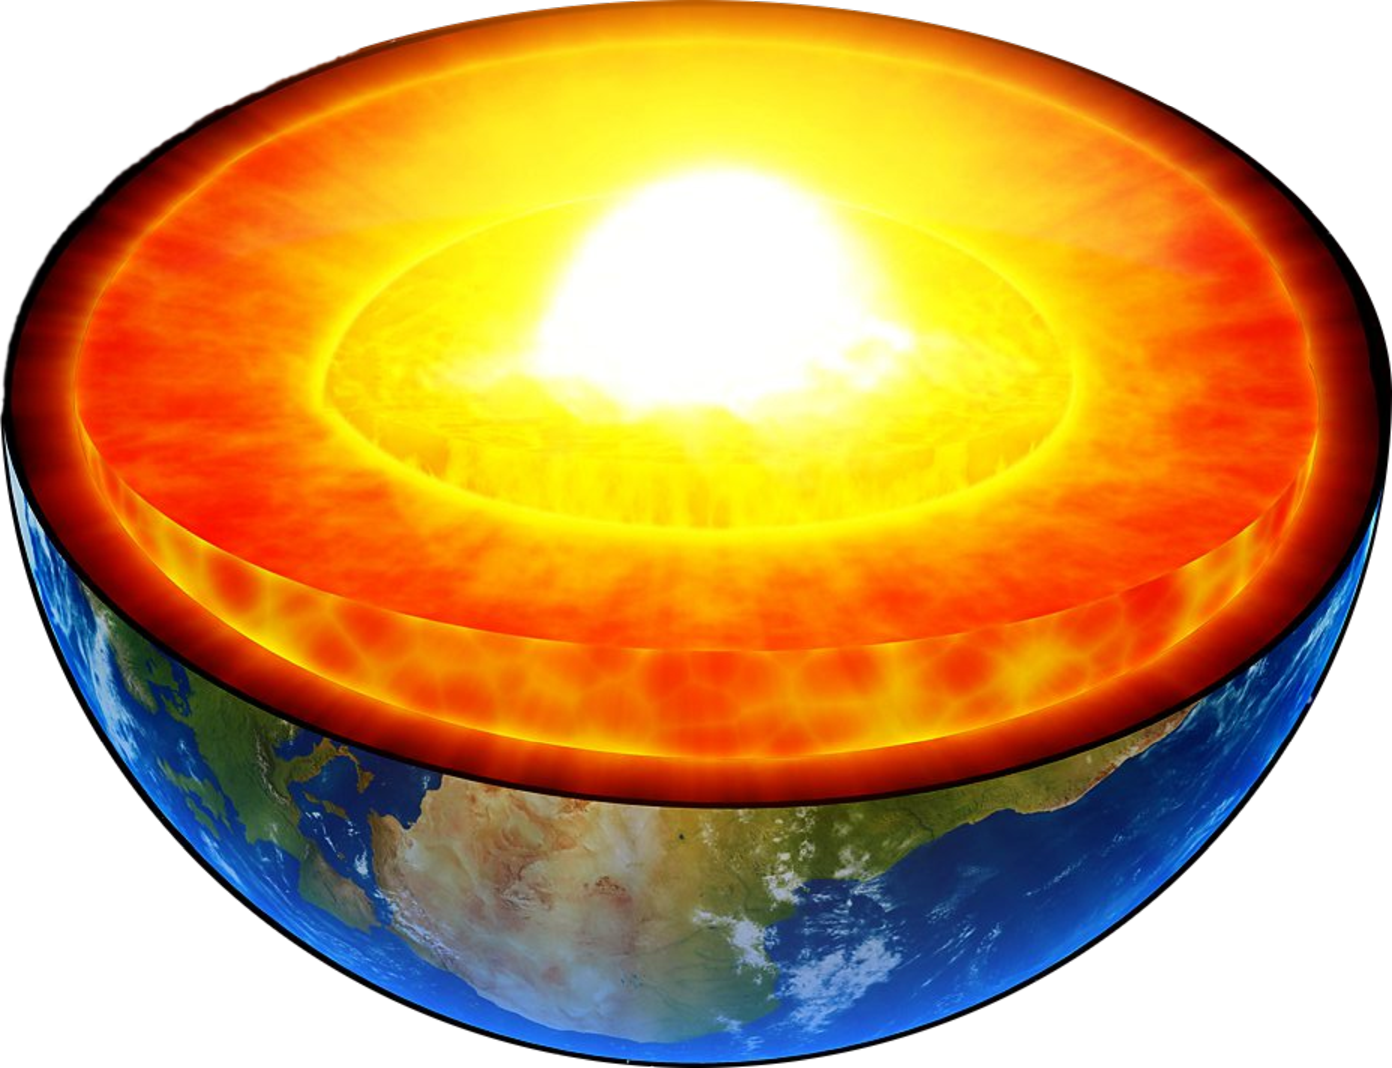
\includegraphics[height=5cm]{figures/terre_core.pdf} 
\end{center} 


\textbf{Résumé :} 
\vspace{0.3cm}

\textbf{Mots clefs :} cailloux, galet de référence
\vspace{0.3cm}


\end{titlepage}

\newpage

\renewcommand\thepage{}

\section*{Remerciements}




\tableofcontents


\newpage
\renewcommand\thepage{\arabic{page}}
\setcounter{page}{1}


\definecolor{linkcolor}{rgb}{0,0,1}

%%%%%%%%%%%%%%%%%%%%%%%%%%%%%%%%%%%%%%%%%%%%%%%%%%%%%%%%%%%%%%%%%%%%%%%%%%%%%%%%%%%%%%%%
%%%%%%%%%%%%%%%%%%%%%%%%%%%%%%%%%%%%%%%%%%%%%%%%%%%%%%%%%%%%%%%%%%%%%%%%%%%%%%%%%%%%%%%%
\section*{Introduction}
%%%%%%%%%%%%%%%%%%%%%%%%%%%%%%%%%%%%%%%%%%%%%%%%%%%%%%%%%%%%%%%%%%%%%%%%%%%%%%%%%%%%%%%%
%%%%%%%%%%%%%%%%%%%%%%%%%%%%%%%%%%%%%%%%%%%%%%%%%%%%%%%%%%%%%%%%%%%%%%%%%%%%%%%%%%%%%%%%
\addcontentsline{toc}{section}{Introduction}


\newpage
%%%%%%%%%%%%%%%%%%%%%%%%%%%%%%%%%%%%%%%%%%%%%%%%%%%%%%%%%%%%%%%%%%%%%%%%%%%%%%%%%%%%%%%%
%%%%%%%%%%%%%%%%%%%%%%%%%%%%%%%%%%%%%%%%%%%%%%%%%%%%%%%%%%%%%%%%%%%%%%%%%%%%%%%%%%%%%%%%
\section{Premiere partie}
%%%%%%%%%%%%%%%%%%%%%%%%%%%%%%%%%%%%%%%%%%%%%%%%%%%%%%%%%%%%%%%%%%%%%%%%%%%%%%%%%%%%%%%%
%%%%%%%%%%%%%%%%%%%%%%%%%%%%%%%%%%%%%%%%%%%%%%%%%%%%%%%%%%%%%%%%%%%%%%%%%%%%%%%%%%%%%%%%

\subsection{Première sous partie}



\section{Quelques formules et notations}
On notera $\partial_x F$ la dérivée partielle telle que $\frac{\partial F}{\partial x}$. On notera $T^t_i$ la valeur de $T$ à $t$ en $r_i$, les $r_i$ appartenant à notre espace discrétisé.


Équation de la chaleur avec terme de production:

\begin{equation}
\rho C_p \partial_t T = \textrm{div} ( k_{T} \vec{\textrm{grad}}(T))  + P
\end{equation}

À 1D cela équivaut à :

\begin{equation}
\rho C_p \partial_t T = \partial_x ( k_{T} \partial_x T)  + P
\end{equation}


 À 3D en supposant une symétrie sphérique on a :

\begin{equation}
\rho C_p \partial_{t'} T' = \frac{1}{r'^2} \partial_{r'} ( k_{T} {r'}^2 \partial_{r'} T')  + P
\end{equation}





On utilisera les formules de discrétisation suivantes :
\begin{align}
\partial_t T &\rightarrow  \frac{T^{t+1}_r - T^{t+1}_r}{\Delta t}\\
\partial_r T &\rightarrow  \frac{T^t_{i+1/2} - T^{t}_{i-1/2}}{\Delta r} \\
\frac{1}{r^2}\partial_r (r^2 \partial_r T ) &\rightarrow \frac{1}{r^2_i \Delta r}\Big [ r^2_{i+1/2}\frac{T^t_{i+1} - T^{t}_{i}}{\Delta r} + r^2_{i-1/2}\frac{T^t_{i-1} - T^{t}_{i}}{\Delta r} \Big]
\end{align}

\section{Modèles}

Note pour tous les modèles suivants on supposera que la Terre est composée d'un mélange homogène de $\phi = $18\% de métal et de 82\% de silicates. Et que les propriétés de ces matériaux ne changent pas avec leur température ou leur changement d'état.

Les constantes respectives et moyennes du mélange sont les suivantes :
\tabulinesep=0.3mm
\begin{center}
  \begin{tabu}{ r | c c c l}
    Grandeur & moyenne & metal & silicate & unité\\ \hline
    Densité ($\rho$) & 4028 & 7800 &  3200 & \SI{}{kg.m^{-3}}\\ \hline
    Capacité calorifique ($C_p$) & 939 & 450 & 1200 &  \SI{}{J.K^{-1}.kg^{-1}} \\ \hline
    Conductivité ($k_T$)& 11.48 & 50 & 3 & \SI{}{W.K^{-1}.m^{-1}}  \\ \hline    
    Chaleur latente de fusion & 413 & 250 & 500 & \SI{}{kJ.kg^{-1}}\\ \hline
    Température de fusion & & 1261 & 1408 & \SI{}{K}\\ \hline

  \end{tabu}
\end{center}

Pour la suite $\rho$ désignera une valeur moyenne et $\rho_{materiau}$ la valeur respective d'un des matériaux.

On utilisera de plus les constantes suivantes :

\begin{center}
  \begin{tabu}{ r  c }
    \hline
    Température initiale & \SI{300}{K}  \\ \hline
    Température de la nébuleuse & \SI{300}{K}  \\ \hline
    Constante de Stephan-Boltzman & \SI{5.67E-8}{W m^{-2} K^{-4}}  \\ \hline
    Demi-vie du $^{26}$Al & \SI{0.717}{My}  \\ \hline
    Abondance du $^{26}$Al & \SI{1.5E-7}{W kg-1}  \\ \hline
  \end{tabu}
\end{center}

\subsection{Modèle 1}

Fichier : sim1.py

\subsubsection{Description}

On fait une première simulation la plus simple possible.
Hypothèses : 
\begin{enumerate}
\item Rayon de la Terre constant 
\item Chauffage causé par la désintégration du $^{26}$Al et par le rayonnement de corps noir à la surface.
\end{enumerate}



\subsubsection{Équations}

On considère les variables adimentionnées suivantes: 


\begin{equation}
t= \frac{t'}{\tau^{Al}_{1/2}}  \quad \textrm{,} \quad   r = r' \sqrt{\frac{\rho C_p} {k_T \tau_{1/2}}} \quad  \textrm{et} \quad T = \frac{T'}{T_{neb}} 
\end{equation}

Il en résulte l'équation suivante :


\begin{equation}
\frac{\rho C_p T_{neb}}{\tau_{1/2}} \partial_{t} T = \frac{\rho C_p T_{neb}}{\tau_{1/2}} \frac{1}{r^2} \partial_{r} ( {r}^2 \partial_{r} T)  + P +( S + Q_L)
\end{equation}


Avec :
\begin{equation}
 P = \rho H_0 e^{-ln(2) t} \quad \textrm{la production de chaleur par radioactivité }
\end{equation}

%Pour passer d'une puissance surfacique à une puissance volumique on introduit 1/delta r
Les termes $S$ et $Q_L$ sont traités séparément de la résolution de l'équation principale, ils représentent: 
\begin{equation}
 S =\frac{\sigma T_{neb}^4}{\Delta r}( 1 - T^4)  \quad \textrm{le rayonnement de corps noir (à la surface uniquement)}
\end{equation}
$Q_L$ représente la chaleur "perdue" lors du changement de phase de chaque matériau. Ce changement de phase est géré en dehors de l'équation de la chaleur. On note $\phi_{met}$ la proportion solide/liquide du métal et $\phi_{sil}$ pour le silicate ($\phi_{sil} = 0 \rightarrow$ solide, $\phi_{sil} = 1 \rightarrow$ liquide). On detecte le changement de phase solide $\rightarrow$ liquide du métal par la condition  $T' > T_{fus,met} $ et $ \phi_{met} < 1$ on "échange" alors de la température contre du changement de phase jusqu'à qu'une des condition de changement d'état atteigne sa limite de validité: c'est à dire soit $T' = T_{fus,met}$ soit $\phi_{met} = 1$. On fait de même avec la transition inverse et avec le silicate.

Exemples : on part de $T' > T_{fus,met}$ , $ \phi_{met} < 1$  \\
\textcolor{red}{!! Attention $T_i$, $T_f$ et $T_{afus}$ sont des variables adimentionées contrairement à $T'$ et $T_{neb}$ !!}


Cas 1 on atteint $\phi_{met} = 1$. Calculons la température finale : 

\begin{equation}
T_{f} =  T_{i} +  (\phi_{met,i} - 1 ) \frac{\phi L_{met}}{T_{neb} C_{p,met} }
\end{equation}

Cas 2 on atteint $T' = T_{fus,met}$. Calculons le $\phi_{met}$ final : 

\begin{equation}
\phi_{f} =  \phi_{i} +  (T_{i}-T_{afus,met}) \frac{T_{neb} C_{p,met}}{\phi L_{met}}
\end{equation}

\subsubsection{Équations discrétisées}

On pose $c_0 = \frac{\Delta t \tau_{1/2} }{\rho C_p T_{neb}}$ 

L'équation adimensionnée peut se réécrire sous la forme de l'équation matricielle suivante :
\begin{equation}
MT^{t+1} = T^t + c_0 ( P + S )
\end{equation}

Avec la matrice $M$ calculée plus tôt : 
$
M = \Big [ Id + \frac{\Delta t ~ r^2_{i+1/2}}{r^2_i \Delta r^2} ~ d1 + \frac{\Delta t ~ r^2_{i-1/2}}{r^2_i \Delta r^2} ~ d2  \Big]
$

\begin{equation}
d1=
\begin{bmatrix}
    2      & -1     & -1        & 0     &\dots      & 0 \\
    0      &  1     & -1        & 0     &           & \vdots  \\
    \vdots & \ddots & \ddots    &\ddots & \ddots    & \vdots \\
    \vdots &        & \ddots    &\ddots & \ddots    & 0 \\
    \vdots &        &           &\ddots & 1         &  -1 \\
    0      & \dots  & \dots     &\dots  & 0         &  0
\end{bmatrix}
d2=
\begin{bmatrix}
     0     & 0      & \dots  & \dots    &\dots      & 0 \\
    -1     & 1      & \ddots &          &           & \vdots  \\
    0      & \ddots & \ddots & \ddots   &           & \vdots \\
    \vdots & \ddots & \ddots & \ddots   & \ddots    & \vdots \\
    \vdots &        & 0      &  -1      &  1        & 0\\
    0      & \dots  & 0      &  -1      & -1        & 2 \\
\end{bmatrix}
\end{equation}


\subsubsection{Résultats}

\begin{figure}
\centering
\begin{subfigure}{.5\textwidth}
  \centering
  
  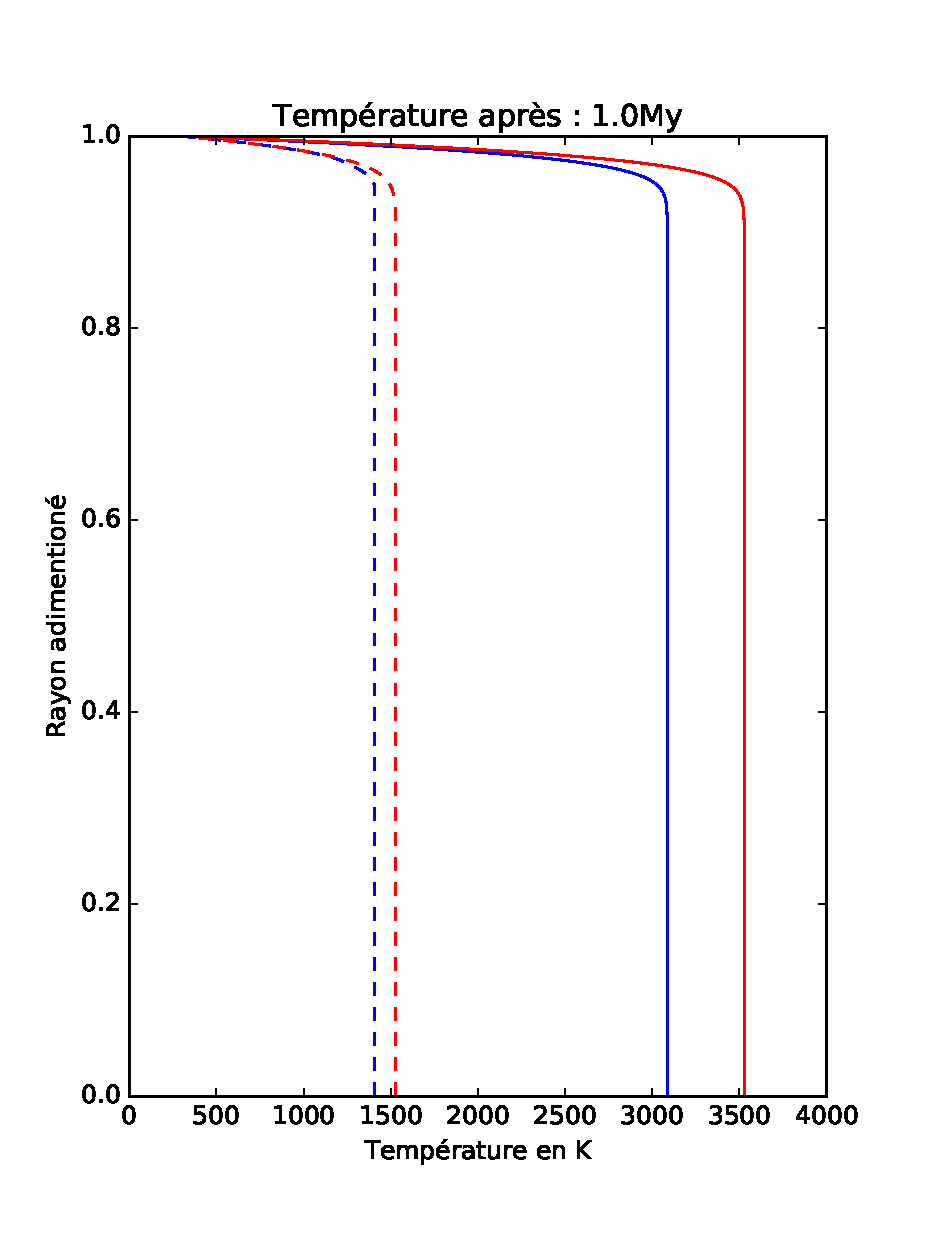
\includegraphics[height=9cm]{./figures/graph_sim1_fig1.eps}
  \caption{}
  \label{fig:sub1}
\end{subfigure}%
\begin{subfigure}{.5\textwidth}
  \centering
  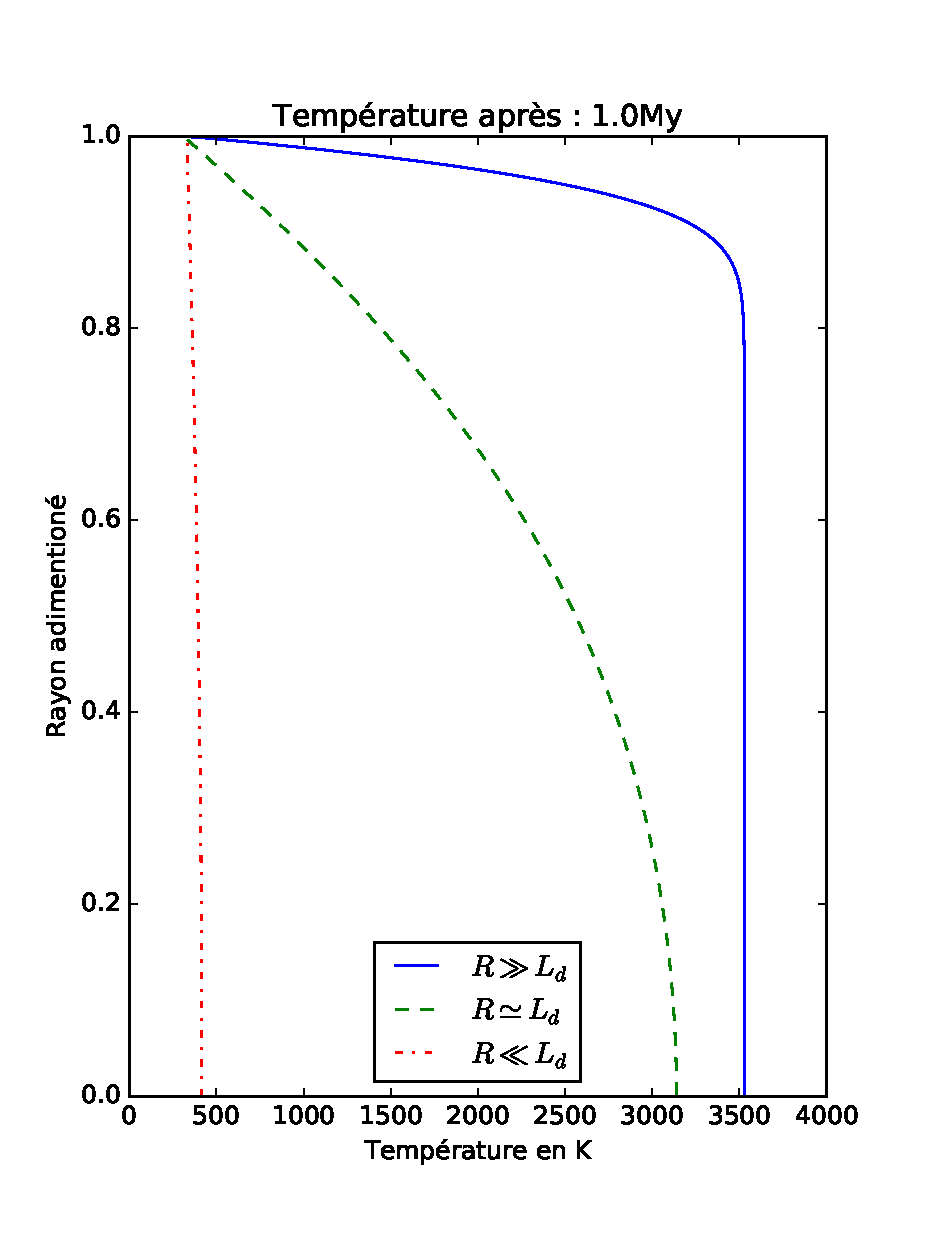
\includegraphics[height=9cm]{./figures/graph_sim1_fig2.eps}
  \caption{}
  \label{fig:sub2}
\end{subfigure}
\caption{On peut voir sur ces figures le profil de température dans une planète après \SI{1}{My} de chauffage par la décomposition radioactive du $^{26}$Al. Sur la figure (a) on peut voir en trait plein le profil en supposant une origine des temps à \SI{0}{My} et en pointillé une origine des temps à \SI{1}{My}, les courbes bleues tiennent compte de la fusion des matériaux et les courbes rouges n'en tienne pas compte. Sur la figure (b) on peut voir le profil de température après \SI{1}{My} selon le rapport entre le rayon de la planète $R$ et la longueur caractéristique de diffusion $L_d \simeq 10 km $. }
\label{fig:test}
\end{figure}

Comme on peut l'observer sur la figure \ref{fig:sub1} lorsqu'on considère un planétésimal de rayon \SI{500}{km}, le profil de température est constant sur 95\% de l'épaisseur de l'astre et chute rapidement quand on approche de la surface. Dans le cas où le chauffage a lieu de manière normale (courbes en trait plein), on constate une augmentation totale de la température d'environ \SI{3527}{K} par rapport à la température initiale de \SI{300}{K} ce qui est proche de \SI{3543}{K}, la température attendue pour un système adiabatique dans les mêmes conditions, quand on ne tient pas compte de la fusion des matériaux (courbes rouges). Si on tient compte de la fusion la température finale est de \SI{3085}{K}, ce qui correspond à la différence attendue d'environ \SI{440}{K} perdus dans la chaleur latente de fusion. Lorsque l'on prend des conditions initiales retardées de \SI{1}{My} (courbes en tirets) les températures finales sont réduites de moitié \textcolor{red}{(la raison de ce calcul est d'illustrer le lien entre le début de la formation des planètes et la formation du soleil  (soleil -> fabrique les elements -> flottent dans l'espace  -> s'agrègent en planètes  après x annèes de décroissance radioactive dans l'espace , donc délai x influe sur T final))} .

Les résultats de ce modèle simple permettent aussi de distinguer plusieurs régimes de diffusion selon le rapport du rayon du planétésimal considéré à la longueur caractérique de diffusion sur l'échelle de temps considérée $L_d = \sqrt{\frac{k_T \tau_{1/2}}{\rho C_p}} \simeq 10 km$. En effet le rayonnement radiatif à la surface étant extrêmement efficace du fait de sa variation en $T^4$, la température de la surface est reste quasiment égale à \SI{300}{K}, la température de la nébuleuse. C'est ensuite l'efficacité de la diffusion de la température dans le planétésimal qui détermine si l'influence de la température de surface reste confinée en surface ou si elle diffuse jusqu'au centre de l'astre. On peut observer ces différents régimes sur la figure \ref{fig:sub2}: pour un rayon petit devant la longueur caractéristique de diffusion, le chauffage radioactif n'a quasiment aucune influence, après \SI{1}{My} la température du centre à augmenté d'environ \SI{100}{K}

\textcolor{red}{C'est la figure (b) la plus intéressante pour le quidam, je trouve. Peut etre fusionner le deux, à voir}

C'est un résultat que l'on attendait aussi qualitativement du fait du rapport qu'il existe entre les termes de production volumiques et surfaciques dans une sphère : la production totale d'énergie totale due aux premiers est proportionnelle à $\frac{4}{3} \pi R^3$ et celle due aux seconds à $4 \pi R^2$. Ainsi le rapport \textit{production volumique/production surfacique} évolue comme $R^3/R^2$ autrement dit comme $R$. Ainsi quand $R \rightarrow 0$ le système est dominé par l'influence du terme surfacique tandis que pour $R \rightarrow +\infty$ c'est l'influence de la production volumique qui domine.

\subsection{Modèle 2}

Fichier : sim2.py

\subsubsection{Description}

Pour cette deuxième simulation on va prendre en compte l’accrétion qui change le rayon de la Terre au cours du temps

Hypothèses : 
\begin{enumerate}
\item Rayon de la Terre évoluant en $\dot{R} \simeq R^\beta$ avec $\beta = 0$, $1$ ou $2$
\item Chauffage causé par la désintégration du $^{26}$Al et par le rayonnement de corps noir.
\end{enumerate}

\subsubsection{Données initiales et constantes}

\begin{center}
  \begin{tabu}{ r  c }
    \hline
    Rayon initial de la Terre & \SI{5}{km} \\ \hline
    Rayon final de la Terre & \SI{500}{km} \\ \hline
    Temps de croissance & \SI{1}{My} ou \SI{5}{My}\\ \hline
  \end{tabu}
\end{center}

\subsubsection{Équations}

On considère les mêmes équations que pour le problème précédent cependant il faut tenir compte de la variation du rayon de Terre en fonction du temps, on introduit pour ce faire une nouvelle variable adimensionnée: 

\begin{equation}
r = \frac{ r'}{R(t)} \quad \textrm{et on conserve} \quad t = \frac{t'}{\tau_{1/2}}    \quad      \textrm{et} \quad T = \frac{T'}{T_{neb}} 
\end{equation}

Que l'on remplace dans l'équation qui tient compte du rayon variable :
\begin{equation}
\rho C_p (\partial_{t'} T' - r \frac{\dot{R}}{R}\partial_{r} T')= \frac{1}{r^2} \partial_{r} ( k_{T} \frac{r^2}{R^2} \partial_{r} T')  + P
\end{equation}

L'équation adimensionnée s'écrit alors :

\begin{equation}
\frac{\rho C_p T_{neb}}{\tau_{1/2}} \partial_{t} T =  \frac{1}{r^2} \partial_{r} ( T_{neb} k_{T} \frac{r^2}{R^2} \partial_{r} T) + \frac{\rho C_p T_{neb}}{\tau_{1/2}} r \frac{\dot{R}}{R}\partial_{r} T + P
\end{equation}

Avec :
\begin{equation}
 P = \rho H_0 e^{-ln(2) t} 
\end{equation}


\subsubsection{Équations discrétisées}






\begin{equation}
T^{t+1} - T^t =  \frac{\tau_{1/2}    k_{T}}{\rho C_p } \frac{\Delta t}{r^2} \partial_{r} ( \frac{r^2}{R^2} \partial_{r} T)  +r \Delta t \frac{\dot{R}}{R}\partial_{r} T + \frac{\tau_{1/2}    \Delta t}{\rho C_p T_{neb} } P
\end{equation}


\begin{multline}
T^{t+1}_i + \frac{\tau_{1/2} k_T \Delta t}{\rho C \Delta r^2 R^2 r^2_i}\Big [ r^2_{i+1/2}(T^{t+1}_{i} - T^{t+1}_{i+1}) + r^2_{i-1/2}(T^{t+1}_{i}- T^{t+1}_{i-1}) \Big] \\
+  \Delta t \frac{ r \dot{R}}{2\Delta r R}\Big [ T^{t+1}_{i-1} - T^{t+1}_{i+1}  \Big] = T^{t}_r  + \frac{\tau_{1/2} \Delta t}{\rho C T_{neb}} P^t_i
\end{multline}






On a l'équation matricielle suivante :
\begin{equation}
\Big [ Id + 
c_1  d_1 +  
c_2  d_2 +
c_3  d_3
 \Big] T^{t+1} = T^t + c_0 P  
\end{equation}

Avec  : 
$c_1 = \frac{\tau_{1/2} k_T \Delta t }{\rho C  }
\frac{r^2_{i+1/2}}{\Delta r^2 R^2 r^2_i}$
, $c_2 = \frac{\tau_{1/2} k_T \Delta t }{\rho C  }
\frac{r^2_{i-1/2}}{\Delta r^2 R^2 r^2_i}$
, $c_3 = \Delta t \frac{ r \dot{R}}{2\Delta r R}$
, $c_0 = \frac{\Delta t \tau_{1/2} }{\rho C_p T_{neb}}$ 

\begin{equation*}
d_1=
\begin{bmatrix}
    2      & -1     & -1        & 0     &\dots      & 0 \\
    0      &  1     & -1        & 0     &           & \vdots  \\
    \vdots & \ddots & \ddots    &\ddots & \ddots    & \vdots \\
    \vdots &        & \ddots    &\ddots & \ddots    & 0 \\
    \vdots &        &           &\ddots & 1         &  -1 \\
    0      & \dots  & \dots     &\dots  & 0         &  0
\end{bmatrix}
d_2=
\begin{bmatrix}
     0     & 0      & \dots  & \dots    &\dots      & 0 \\
    -1     & 1      & \ddots &          &           & \vdots  \\
    0      & \ddots & \ddots & \ddots   &           & \vdots \\
    \vdots & \ddots & \ddots & \ddots   & \ddots    & \vdots \\
    \vdots &        & 0      &  -1      &  1        & 0\\
    0      & \dots  & 0      &  -1      & -1        & 2 \\
\end{bmatrix}
d_3=
\begin{bmatrix}
     2     & -2     & 0      & \dots    &\dots      & 0 \\
     1     & 0      & -1     & \ddots   &           & \vdots  \\
    0      & \ddots & \ddots & \ddots   & \ddots    & \vdots \\
    \vdots & \ddots & \ddots & \ddots   & \ddots    & 0 \\
    \vdots &        & \ddots &   1      &  0        & -1\\
    0      & \dots  & \dots  &   0      &  2        & -2 \\
\end{bmatrix}
\end{equation*}


\subsubsection{Résultats}

On peut observer sur la figure \ref{fig2} les conséquences de l'évolution du rayon du planétésimal au cours du temps sur le profil de température. On constate sur la figure \ref{fig2:1} qu'une croissance linéaire du rayon ($\beta=0$) sur un temps comparable au temps de demi-vie du $^{26}$Al (\SI{0.717}{My}) donne un profil qui atteint une température maximale de \SI{3000}{K} proche des \SI{3100}{K} atteint dans notre premier modèle, le profil évolue ensuite linéairement jusqu'à atteindre \SI{300}{K} à la surface. Dans le cas où la croissance est plus accélérée, comme on peut le voir sur la figure \ref{fig2_3}, il est possible de distinguer deux périodes dans l'histoire du planétésimal: une première période de croissance lente avec un rayon faible durant laquelle l'influence des pertes radiatives est grande, suivie d'une inflation très rapide de l'astre où il acquiert la plupart de son épaisseur. La température de l'épaisseur crée lors de cette deuxième phase reste proche de \SI{300}{K} puisque l'intensité du chauffage radioactif à déjà eu le temps, au cours de la première période, de diminuer de moitié dans le cas d'une croissance en \SI{1}{My} et de s'épuiser totalement dans le cas de la croissance en \SI{5}{My} du fait de la demi-vie de \SI{0.717}{My} du $^{26}$Al. On relève au centre des planétésimaux les températures suivantes : \SI{3600}{K}, \SI{950}{K} et \SI{400}{K} pour $\beta$ valant respectivement $0$, $1$ et $2$.

Dans le cas étudié par sur la figure \ref{fig2:2}, la croissance du rayon se fait sur \SI{5}{My}, cette croissance plus lente implique que le planétésimal passe plus de temps dans le régime où la chaleur est rapidement diffusée vers la surface. De ce fait, le chauffage initial est moins efficace et la température du centre croit moins que dans le cas précédent. On relève \SI{3600}{K}, \SI{950}{K} et \SI{400}{K} pour $\beta$ valant respectivement $0$, $1$ et $2$. 

\begin{figure}[h!]
\centering
\begin{subfigure}{.5\textwidth}
  \centering
  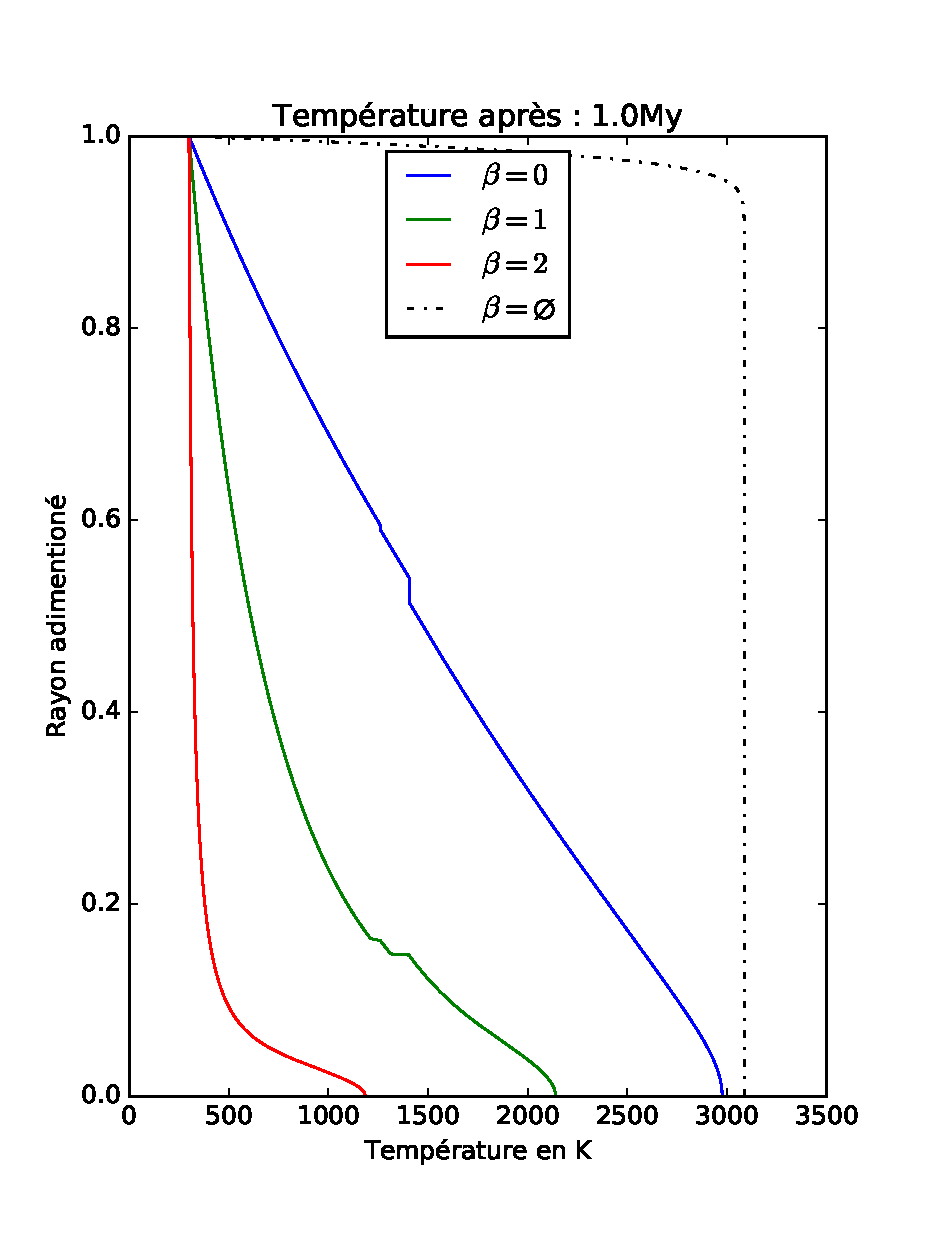
\includegraphics[height=9cm]{./figures/graph_sim2_fig2_1.eps}
  \caption{}
  \label{fig2:1}
\end{subfigure}%
\begin{subfigure}{.5\textwidth}
  \centering
  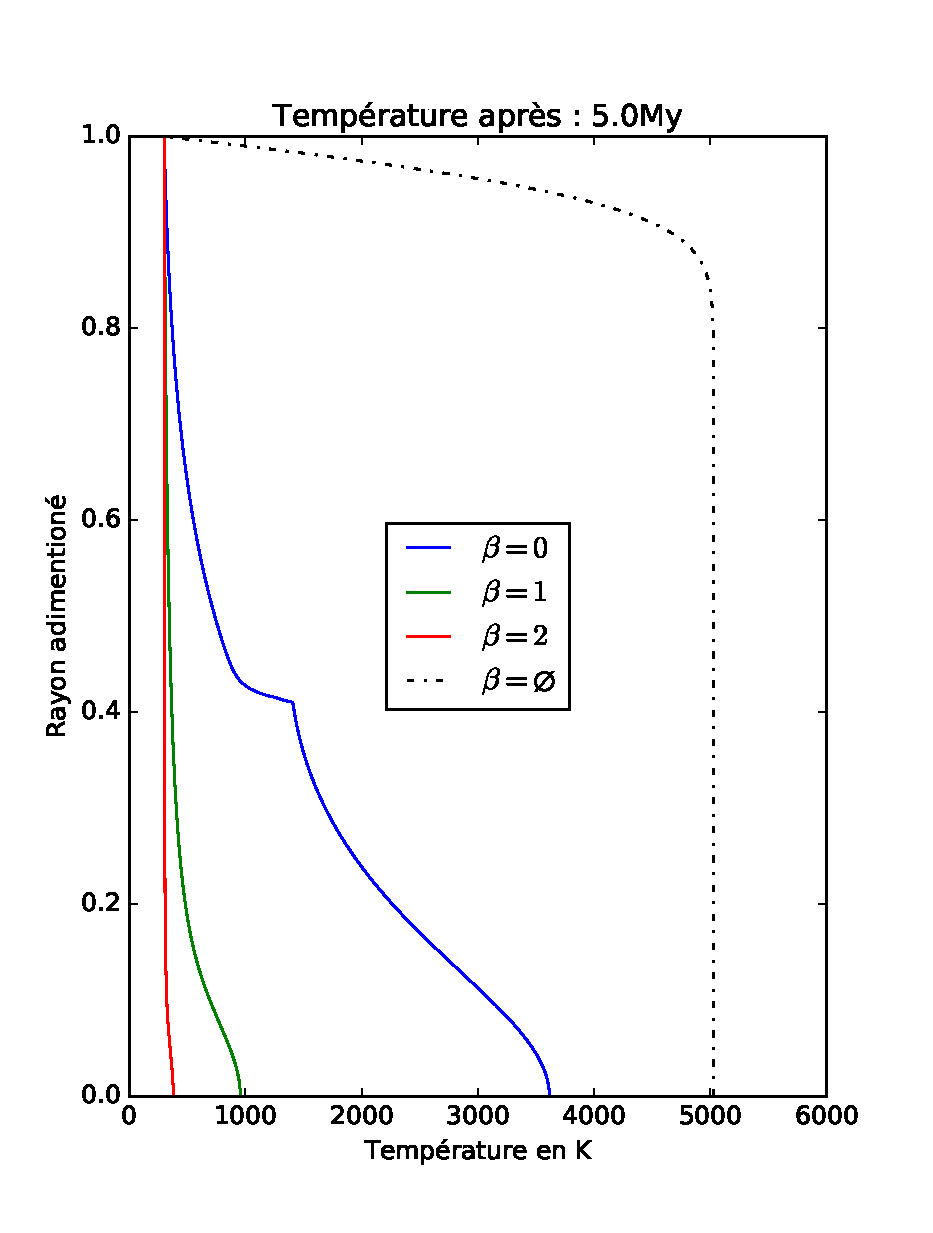
\includegraphics[height=9cm]{./figures/graph_sim2_fig2_2.eps}
  \caption{}
  \label{fig2:2}
\end{subfigure}
\caption{Profil de température dans une planète qui croît par accrétion de \SI{5}{km} à \SI{500}{km} sur une période de \SI{1}{My} sur la figure (a) et de \SI{5}{My} sur la figure (b). Chaque courbe correspond à un taux de croissance différent, les courbes en pointillé  correspondent à un astre dont le rayon est constant à \SI{500}{km} }
\label{fig2}
\end{figure}


\begin{figure}[h!]
\centering
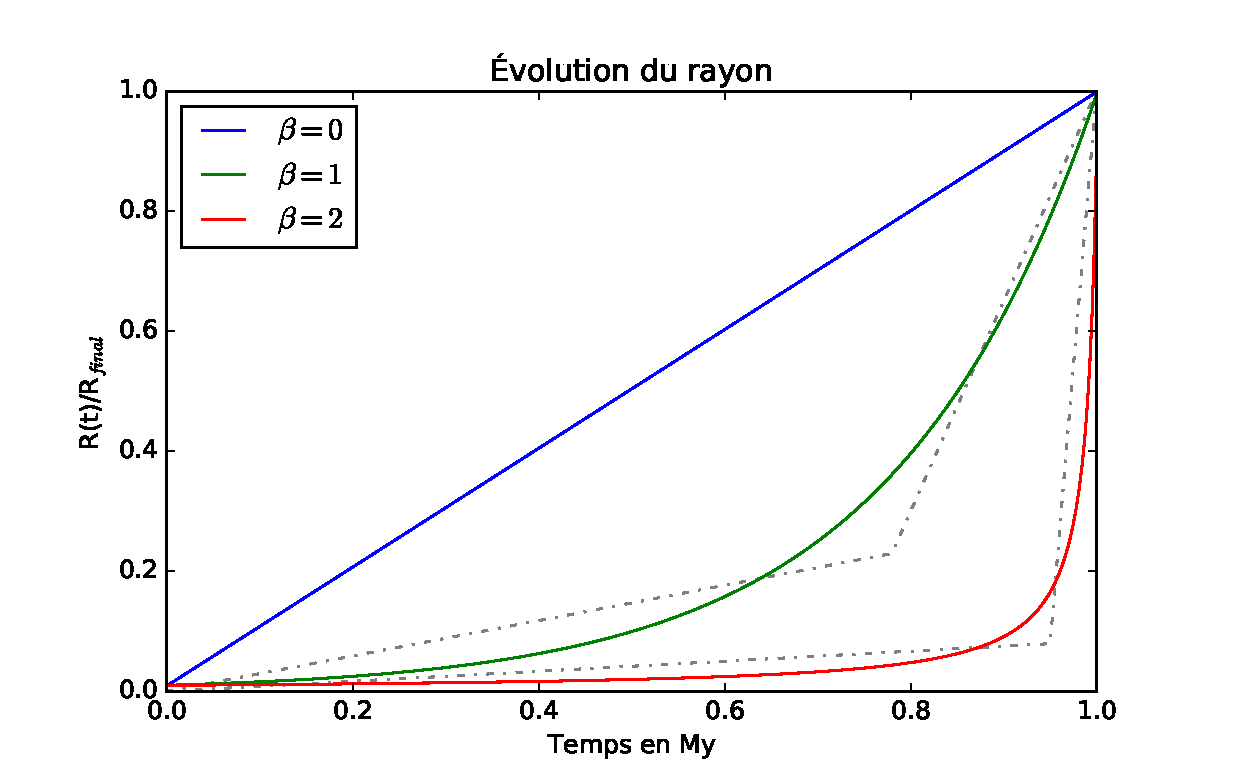
\includegraphics[height=7cm]{./figures/graph_sim2_fig2_3.eps}
\caption{Croissance du rayon en fonction du temps et selon le paramètre $\beta$. On notera que le temps est donné à titre indicatif, en effet le profil de croissance est identique quelque soit l'échelle de croissance choisie. Pour $\beta=1$ et $\beta=2$ les deux régimes de croissances (symbolisé par les courbes pointillées) que l'on peut distinguer sont une croissance lente jusqu'à \SI{0.8}{My} pour $\beta=1$  et \SI{0.95}{My} pour $\beta=2$ suivie d'une croissance rapide jusqu'au rayon final en \SI{0.2}{My} et \SI{0.05}{My} respectivement.}
\label{fig2_3}
\end{figure}


\subsection{Modèle 3}

Fichier : sim3.py

\subsubsection{Description}

On reprend la physique du modèle 2 en tenant compte cette fois de l'apport de chaleur qui résulte des impacts. Cette chaleur provient à la fois de la température propre du corps impactant et de l'énergie cinétique de ce dernier, acquise du fait de l'attraction entre le planétésimal et le corps impactant. L'impact ne permet toutefois pas au planétésimal de récupérer l'intégralité de l'énergie de l'impactant, seule une portion $f=20-40\%$ étant capturée et le restant étant immédiatement perdu par rayonnement. On comparera plusieurs possibilité sur la température de ces corps impactants.

Hypothèses : 
\begin{enumerate}
\item Rayon de la Terre évoluant en $\dot{R} \simeq R^\beta$ avec $\beta = 0$, $1$ ou $2$
\item Chauffage causé par la désintégration du $^{26}$Al, par le rayonnement de corps noir et par la déposition d'une fraction $f=20\%$ de l'énergie propre des corps impactants.
\item La taille moyenne des impactants évolue proportionnellement au rayon du planétésimal et vaut $R(t)/5$.
\item Le chauffage provoqué par l'impact se fait uniformément dans un couche d'épaisseur $\Delta R = R(t)/5$ à la surface.
\item La température de l'impactant sera supposé soit constante égale à \SI{1000}{K} soit variable estimée à partir du modèle 2.
\end{enumerate}

\subsubsection{Données initiales et constantes}

\begin{center}
  \begin{tabu}{ r  c }
    \hline
    Rayon initial de la Terre & \SI{5}{km} \\ \hline
    Rayon final de la Terre & \SI{500}{km} \\ \hline
    Temps de croissance & \SI{1}{My} ou \SI{5}{My}\\ \hline
    Fraction d'énergie déposée & 20\%       \\ \hline
  \end{tabu}
\end{center}

\subsubsection{Équations}

\begin{equation}
\frac{\rho C_p T_{neb}}{\tau_{1/2}} (\partial_{t} T -  r \frac{\dot{R}}{R} \partial_{r} T)= \frac{\rho C_p T_{neb}}{\tau_{1/2}} \frac{1}{r^2} \partial_{r} ( {r}^2 \partial_{r} T)  + P + H_g
\end{equation}
Avec :
\begin{equation}
 P = \rho H_0 e^{-ln(2) t} 
\end{equation}
et sur la couche $\Delta R$:
 
\begin{align}
 &H_g = \frac{f}{4 \pi R^2 \Delta R}(\partial_{t} E_g + \partial_{t} E_t) \\
 &\partial_{t} E_g =\frac{16}{3} \pi^2 G \rho^2 R^4 \dot R \\
 &\partial_{t} E_t = 4 \pi \rho C_p ( T_{imp} - T_{neb} ) R^2 \dot R
\end{align}


\begin{equation}
H_g = f \frac{4 \pi}{3} G \rho^2 \frac{R^2\dot R}{\Delta R} + f \rho C_p \frac{\dot R}{\Delta R} ( T_{imp} - T_{neb} )
\end{equation}


\subsubsection{Équations discrétisées}

L'équation matricielle du modèle précédent reste valable, on doit juste ajouter le terme de production supplémentaire :
\begin{equation}
\Big [ Id + 
c_1  d_1 +  
c_2  d_2 +
c_3  d_3
 \Big] T^{t+1} = T^t + c_0 (P + H_g(r))
\end{equation}

Les matrices $d1$, $d2$ et $d3$ sont inchangée et on rappelle la valeur des coefficients : \\
$c_1 = \frac{\tau_{1/2} k_T \Delta t }{\rho C  }
\frac{r^2_{i+1/2}}{\Delta r^2 R^2 r^2_i}$
, $c_2 = \frac{\tau_{1/2} k_T \Delta t }{\rho C  }
\frac{r^2_{i-1/2}}{\Delta r^2 R^2 r^2_i}$
, $c_3 = \Delta t \frac{ r \dot{R}}{2\Delta r R}$
, $c_0 = \frac{\Delta t \tau_{1/2} }{\rho C_p T_{neb}}$ 



%%%%%%%%%%%%%%%%%%%%%%%%%%%%%%%%%%%%%%%%%%%%%%%%%%%%%%%%%%%%%%%%%%%%%%%%%%%%%%%%%%%%%%%%
%%%%%%%%%%%%%%%%%%%%%%%%%%%%%%%%%%%%%%%%%%%%%%%%%%%%%%%%%%%%%%%%%%%%%%%%%%%%%%%%%%%%%%%%
\section*{Conclusion}




%%%%%%%%%%%%%%%%%%%%%%%%%%%%%%%%%%%%%%%%%%%%%%%%%%%%%%%%%%%%%%%%%%%%%%%%%%%%%%%%%%%%%%%%
%%%%%%%%%%%%%%%%%%%%%%%%%%%%%%%%%%%%%%%%%%%%%%%%%%%%%%%%%%%%%%%%%%%%%%%%%%%%%%%%%%%%%%%%
\addcontentsline{toc}{section}{Conclusion}


\newpage
%%%%%%%%%%%%%%%%%%%%%%%%%%%%%%%%%%%%%%%%%%%%%%%%%%%%%%%%%%%%%%%%%%%%%%%%%%%%%%%%%%%%%%%
%%%%%%%%%%%%%%%%%%%%%%%%%%%%%%%%%%%%%%%%%%%%%%%%%%%%%%%%%%%%%%%%%%%%%%%%%%%%%%%%%%%%%%%
\appendix
%%%%%%%%%%%%%%%%%%%%%%%%%%%%%%%%%%%%%%%%%%%%%%%%%%%%%%%%%%%%%%%%%%%%%%%%%%%%%%%%%%%%%%%
%%%%%%%%%%%%%%%%%%%%%%%%%%%%%%%%%%%%%%%%%%%%%%%%%%%%%%%%%%%%%%%%%%%%%%%%%%%%%%%%%%%%%%%
\section{Première annexe} \label{annexe_fonctionnelles}
$ \rho L \frac{\partial \phi}{\partial t} = \rho L \frac{d \phi}{d T}\frac{\partial T}{\partial t} $ avec $\phi$ qui est une marche, on peut l'approximer par une fonction un peu plus dérivable par ex :  $\phi \simeq arctan(T-T_{fusion})$ 

$ \rho Cp_{eff} = \rho Cp(\phi) + \rho L  \frac{d \phi}{d T}$



$R_T = a t^b , T = T(t,r/R_T(t)) $

$\Rightarrow \frac{\partial T(t,r/R_T(t))}{\partial t}  = \frac{\partial T}{\partial t} + \frac{\partial \frac{r}{R_T(t)}}{\partial t}\frac{\partial T}{\partial r} = \frac{\partial T}{\partial t} + \frac{\partial \frac{r}{R_T(t)}}{\partial t}\frac{\partial T}{\partial r} $


\subsubsection{autre méthode possible (en fait pas besoin de ca)}


On peut essayer de traiter le problème en deux temps : 

\begin{equation}
\frac{ dT'}{dt'} = \partial_{t'} T' + \frac{\partial r'}{\partial t'} \partial_{r'} T' = \partial_{t'} T' + r \frac{\dot{R}}{R}\partial_{r} T'
\end{equation}

où $r'(t) = R(t)r$ avec $r \in [0,1]$

\tikzstyle{int}=[draw, fill=blue!20, minimum size=2em]
\tikzstyle{init} = [pin edge={to-,thin,black}]

\begin{tikzpicture}[node distance=2.5cm,auto,>=latex']
    \node[below left] (a) {$T'_{t}$};
    \node[below left,right of=a] (b) {$\tilde{T}'_{t+1}$};
    \node[below left,above of=b] (c) {$T'_{t+1}$};
    \path[->] (a) edge node {$\frac{ dT'}{dt'}$} (c);
    \path[->] (a) edge node [below] {$\partial_t' T'$} (b);
    \path[->] (b) edge node [right] {$r \frac{\dot{R}}{R}\partial_{r} T'$} (c) ;
\end{tikzpicture}

On calcule donc d'abord une première estimation de la température $\tilde{T}'_{t+1}$ avec uniquement les contributions diffusives :

\begin{equation}
\rho C_p \partial_{t'} T'= \rho C_p \frac{\tilde{T}'_{t+1} - T'_{t}}{\Delta t'} = \frac{1}{r^2} \partial_{r} ( k_{T} \frac{r^2}{R^2} \partial_{r} T')  + P
\end{equation}

On calcule a partir de cette température intermédiaire la contribution du terme de transport pour avoir la température finale:

\begin{equation}
\frac{T'_{t+1} - T'_{t}}{\Delta t'} = \frac{\tilde{T}'_{t+1} - T'_{t}}{\Delta t'} + \frac{\partial r'}{\partial t'} \partial_{r'} T' =  \frac{\tilde{T}'_{t+1} - T'_{t}}{\Delta t'} + \frac{r\Delta R}{R\Delta t'}\partial_{r} T'
\end{equation}

D'où

\begin{equation}
T'_{t+1}  = \tilde{T}'_{t+1} + \frac{r\Delta R}{R}\partial_{r} T'_{t+1}
\end{equation}

On résout à la suite ces deux équations matricielles :

\begin{equation}
\left\{
\begin{array}{r c l}
M_1 \tilde{T}'_{t+1} &=& T'_t + c_0 ( P + S )\\
M_2 T'_{t+1}   &=& \tilde{T}'_{t+1}\\
\end{array}
\right.
\end{equation}

\newpage
\bibliographystyle{unsrt}
\bibliography{rapport} 
\addcontentsline{toc}{section}{Références} 


\end{document}
